\subsection{Static verification}
	With all the geometrical values known, it has been possible to carry out a more detailed analysis. Considering a more complex model of the forces that takes into account also the distributed load due to the gravity and that the force $F$ is applied with an eccentricity $e=5cm$, it has been possible to parametrically define the hyperstatic variables as
	\[ X_1 \simeq \big( 0.63-0.16\zeta\big) N\cdot m \qquad X_2 \simeq -8.10 \ N\cdot m \] \[ X_3 \simeq \big( - 10.54 - 11.07\zeta + 55.53\zeta^2 - 6.17\zeta^3 \big) N\cdot m \]
	Evaluating the stress state on the 3 beams making up the structure for values of $\zeta \in [0,L]$, what we obtained is that the most critical section is in the elevated track for $\zeta^* = 1.65m$ at $z^* = 1.65m$ where the maximum bending value $M_x^* \simeq 135.64N\cdot m$ is achieved (as showed in figure \ref{fig:bending}). Knowing that $N^* = 0$ and neglecting the shear stress contribution due to both shear $V_y^* \simeq 111N$ and torque $M_z^* \simeq 1.89N\cdot m$, the stress state is
	\[ \sigma_{zz}(y) = \frac{M_x^*}{I_{xx,track}}y \qquad \Rightarrow \qquad \sigma_{zz,max} = \sigma_{zz}(2cm) \simeq 28.68 MPa   \]
	\begin{figure}[b]
		\centering 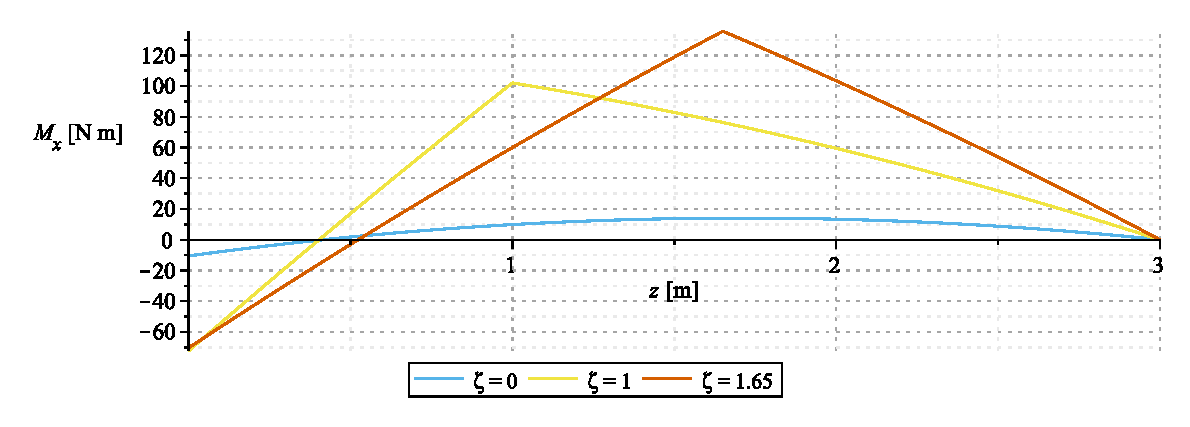
\includegraphics[width=\linewidth]{bending}
		\caption{bending moment $M_x$ acting along the elevated track for 3 values o application point of the force; the first case is the minimum-stress condition, while the third one has the maximum bending peek value.} \label{fig:bending}
	\end{figure}
	This leads to a safety factor of $\phi = \sigma_{ys}/\sigma_{zz,max} \simeq 8.37$, meaning that the structure is statically verified. This value is more then twice than the one achieved in the preliminary design phase but is due to the fact that in this case the full analytical solution of the hyperstatic problem has been considered, having determined all geometrical properties of the sections. As a reminder:
	\begin{itemize}
		\item due to the lack of analytical formulas for such complex geometry section, shear components due to torque and shears are neglected and could have influenced the mechanical system;
		\item we did not consider external forces acting that might act on the global $x$ axis due to the actuation of the machine or accidental load applied by the end user: this can lead to an increase in bending and torques that might make the system fail; a high safety factor ensures us the reliability of the system also in such conditions.
	\end{itemize}
	
	\textbf{AGGIUNGERE LA STIFFNESS VERIFICATION}